\chapter{Технологический раздел}
\label{cha:impl}
В данном разделе описываются технические средства, используемые при проектировании распределенной системы обработки информации. Также приведены результаты разработки системы.

\section{Среда разработки и язык программирования}
Разработка РСОИ осуществлялась на языке Python.
Выбор данного языка программирования обусловлен платформонезависимостью, большим количеством своих и сторонних библиотек, а также наличием его в списке рекомендуемых кафедрой.

В качестве дополнительных иблиотек использовались:
\begin{enumerate}
\item CherryPy — объектно-ориентированный веб-фреймворк, написанный на языке программирования Python. Спроектирован для быстрой разработки веб-приложений для сети Интернет. Представляет собой надстройку над HTTP-протоколом, но остаётся на низком уровне и не выходит за рамки требований RFC 2616.
\item SQLAlchemy - программная библиотека на языке Python для работы с реляционными СУБД с применением технологии ORM. 
\end{enumerate}

В качестве СУБД использовался sqlite - легковесная встраиваемая реляционная база данных, модуль которой встроен в Python по-умолчанию.

\section{Выбор протоколов взаимодействия}
\subsection{Протокол асинхронного взаимодействия}
В качестве протокола асинхронного взаимодействия были выбраны протоколы SMTP/POP3, так как они есть в списке рекомендуемых кафедрой протоколов для выполнения курсового проектирования.

\subsection{Протокол синхронного взаимодействия}
В качестве протокола синхронного взаимодействия был использован протокол HTTP.

\section{Диаграммы классов}
\subsection{Диаграмма классов системы кадрового агентства}
Диаграмма классов представлена на рисунке ~\ref{fig:Visio-hh-uml}.

\begin{figure}[ht!]
\centering
 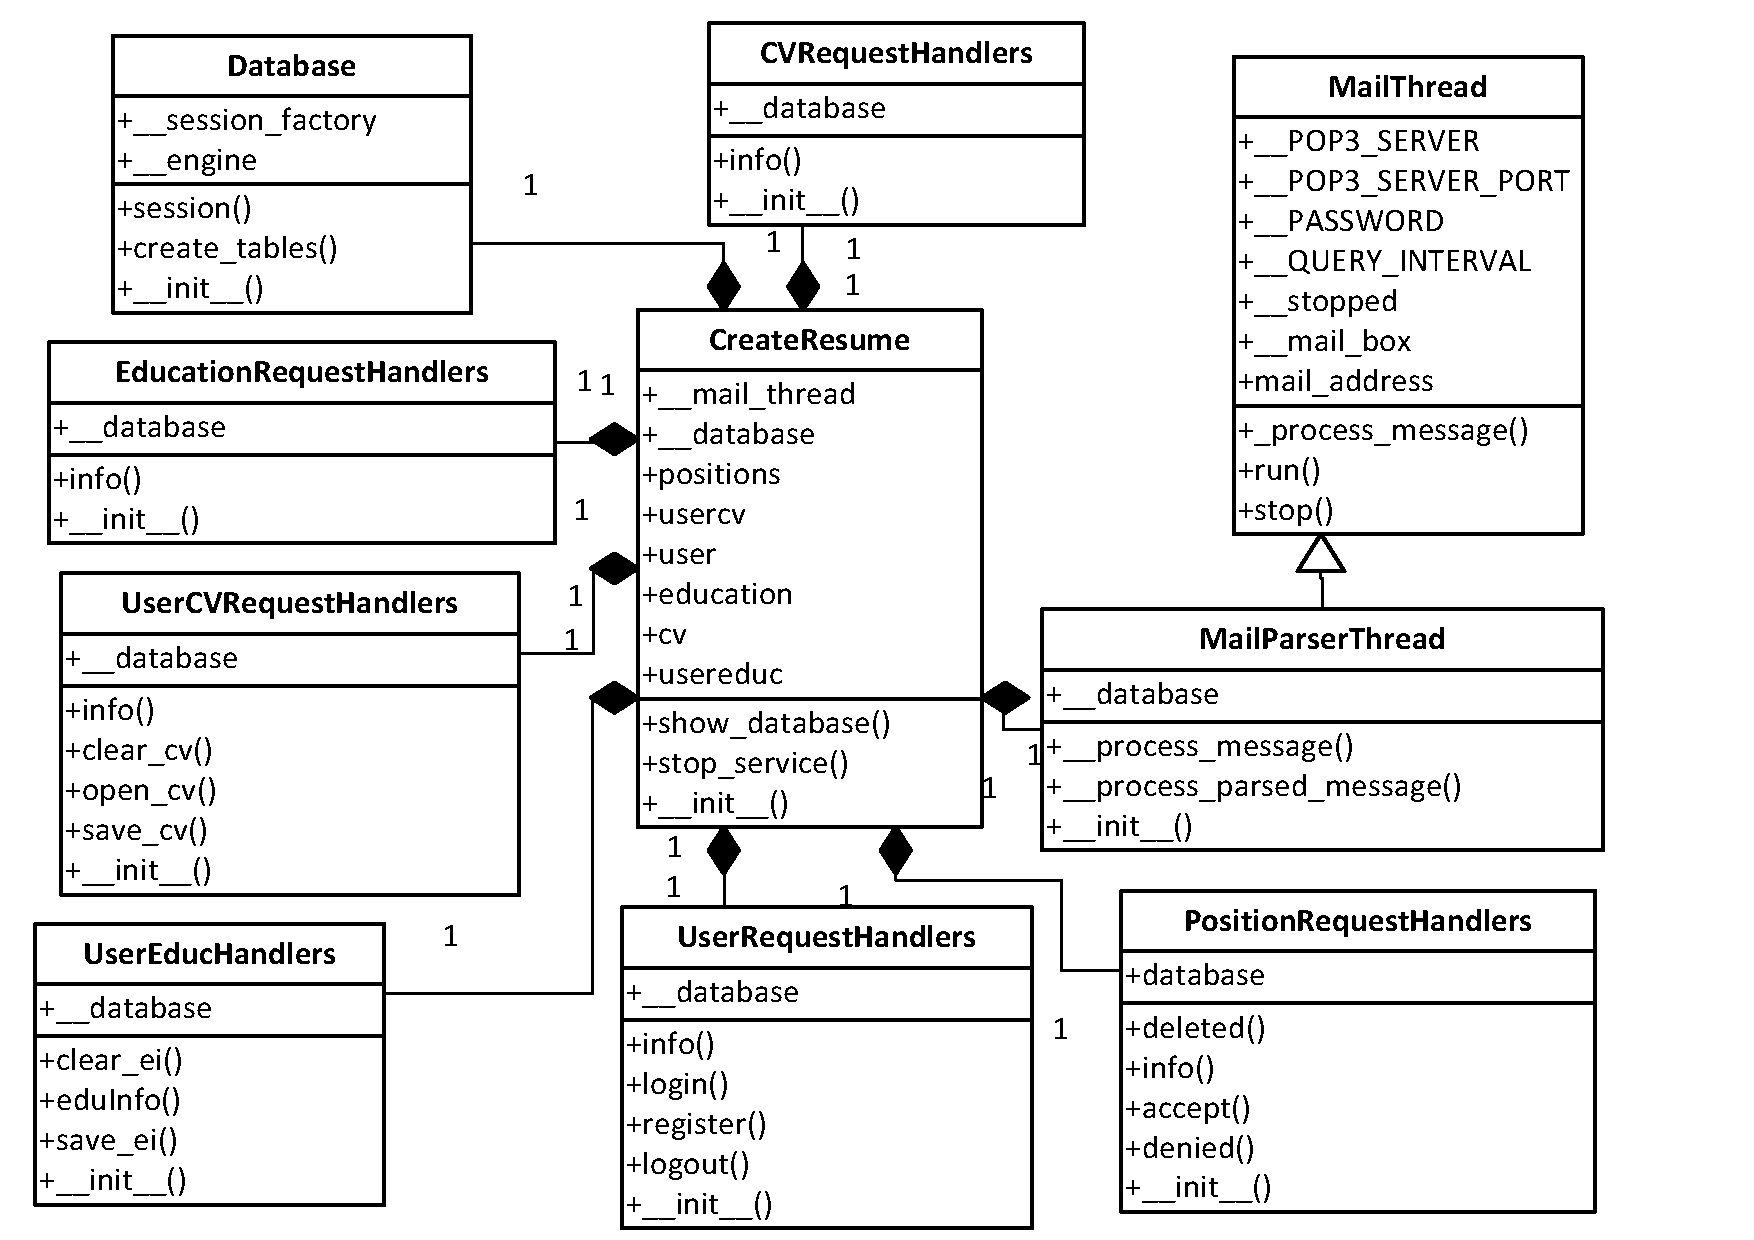
\includegraphics[width=\textwidth]{include/Visio-hh-uml.pdf}
\caption{Диаграмма классов системы кадрового агентства}
\label{fig:Visio-hh-uml}
\end{figure}

Ниже приведена спецификация классов системы кадрового агентства.

\textbf{Спецификация классов системы кадрового агентства}
\begin{enumerate}
\item EducationRequestHandlers – класс, выполняющий отправку списка возможных параметров образования в веб-интерфейс.
	\begin{enumerate}
	\item info – метод возвращает все возможные списочные параметры образования, такие как университет, тип обучения, иностранные языки и уровень их знаний, в формате JSON;
	\end{enumerate}
\item CvRequestHandlers – класс, выполняющий отправку списка возможных параметров резюме в веб-интерфейс.
	\begin{enumerate}
	\item info – метод возвращает все возможные списочные параметры резюме, такие как график работы, график командировок и отрасль, в формате JSON;
	\end{enumerate}
\item UserRequestHandlers – класс, выполняющий обработку запросов, поступающих с веб-интерфейса, касающихся регистрации, аутентификации и получении имени текущего пользователя.
	\begin{enumerate}
	\item info – метод возвращает полное имя пользователя в формате JSON;
	\item login – метод принимает email и пароль пользователя производит аутентификацию;
	\item register – метод принимает данные пользователя в том числе email и пароль и регистрирует в системе;
	\item logout – метод завершает сессию для пользователя.                  
	\end{enumerate}
\item UserEducHandlers – класс, выполняющий обработку запросов, поступающих с веб-интерфейса, касающихся образования пользователя.
	\begin{enumerate}
	\item clear_ei - метод удаляет все возможные данные об образовании данного пользователя;
	\item save_ei - метод принимает данные об образовании из веб-интерфейса и сохраняет их;
	\item eduInfo - метод возвращает данные об образовании пользователя в формате JSON;
	\end{enumerate}
\item UserCvHandlers – класс, выполняющий обработку запросов, поступающих с веб-интерфейса, касающихся критериев, указываемых в резюме.
	\begin{enumerate}
	\item clear_cv - метод удаляет все возможные резюме данного пользователя;
	\item save_cv - метод принимает данные о резюме из веб-интерфейса и сохраняет их в базе кадрового агентства;	
	\item open_cv - метод отправляет критерии, взятые из резюме, соответствующей отраслевой организации;
	\item info - метод возвращает список резюме данного пользователя;
	\end{enumerate}
\item PositionRequestHandlers – класс, выполняющий обработку запросов, поступающих с веб-интерфейса, касающихся отобранных для пользователя вакансий.
	\begin{enumerate}
	\item deleted - метод удаляет позицию из базы кадрового агентства;         
	\item info - метод возвращает список доступных вакансий в формате JSON;    
	\item accept - метод, вызываемый при принятии пользователем текущего предложения, меняется статус вакансии в базе, соответствующее сообщение отсылается в отраслевое агенство;         
	\item denied - метод, вызываемый при отказе пользователя рассматривать данную вакансию, после этого позиция доступна только для удаления, в базе ставится соответствующий статус вакансии, данные отсылаются в отраслевую организацию;         
	\end{enumerate}
\item MailThread – класс, реализующий прием электронных писем по протоколу POP3.
	\begin{enumerate}
	\item _process_message – метод, переопределяемый в классах-потомках;                                                                   
	\item run – метод запускающий процесс периодической проверки почтового ящика;
	\item stop – метод останавливающий процесс периодической проверки почтового ящика;
	\end{enumerate}
\item MailParserThread – класс, унаследованный от MailThread, обрабатывает входящие электронные письма.
	\begin{enumerate}
	\item _process_message - метод принимающий письма и получающий из них отправителя и содержимое;     
	\item \underline{ }\underline{ }process_parsed_message - метод обрабатывающий содержимое писем и, в соответствии с полученными данными, изменяющий информацию о доступных вакансиях;
	\end{enumerate}
\item Database – класс, реализующий прием электронных писем по протоколу POP3.
	\begin{enumerate}
	\item create_tables – метод, создающий таблицы из метаданных объектов;
	\item session – метод, сбрасывает все оставшиеся изменения в базу и фиксирует транзакции, в случае неудачи откатывает сессию;
	\end{enumerate}	
\end{enumerate}

\subsection{Диаграмма классов системы компании-нанимателя}
Диаграмма классов для компании-нанимателя представлена на рисунке ~\ref{fig:Visio-cmp-uml}.

\begin{figure}[ht!]
\centering
 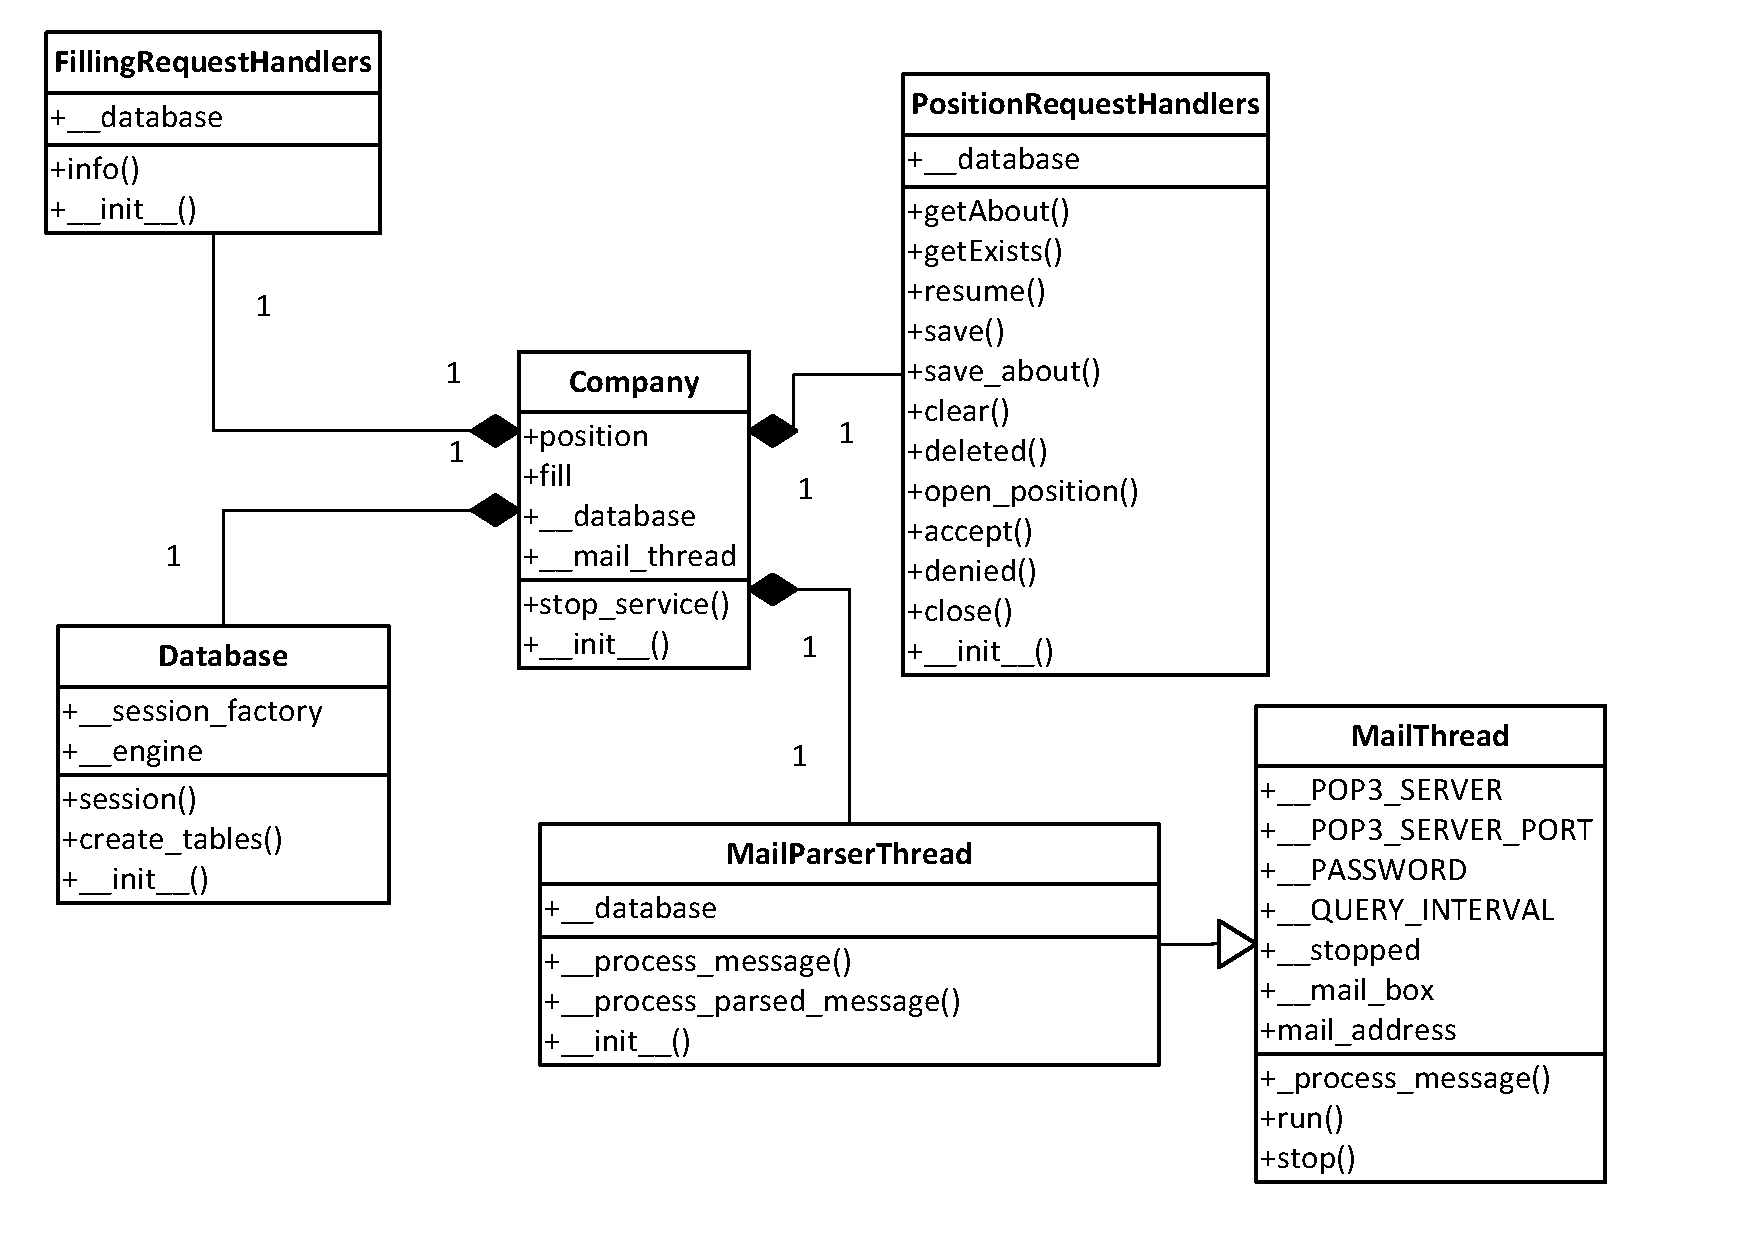
\includegraphics[width=\textwidth]{include/Visio-cmp-uml.pdf}
\caption{Диаграмма классов системы компании-нанимателя}
\label{fig:Visio-cmp-uml}
\end{figure}

Ниже приведена спецификация классов компании-нанимателя.

\textbf{Спецификация классов компании-нанимателя}
\begin{itemize}
\item Database – класс, реализующий прием электронных писем по протоколу POP3.
	\begin{itemize}
	\item create_tables – метод, создающий таблицы из метаданных объектов;
	\item session – метод, сбрасывает все оставшиеся изменения в базу и фиксирует транзакции, в случае неудачи откатывает сессию;
	\end{itemize}	
\item MailThread – класс, реализующий прием электронных писем по протоколу POP3.
	\begin{itemize}
	\item _process_message – метод, переопределяемый в классах-потомках;                                                                   
	\item run – метод запускающий процесс периодической проверки почтового ящика;
	\item stop – метод останавливающий процесс периодической проверки почтового ящика;
	\end{itemize}
\item MailParserThread – класс, унаследованный от MailThread, обрабатывает входящие электронные письма.
	\begin{itemize}
	\item _process_message - метод принимающий письма и получающий из них отправителя и содержимое;     
	\item \underline{ }\underline{ }process_parsed_message - метод обрабатывающий содержимое писем и, в соответствии с полученными данными, изменяющий информацию о доступных вакансиях;
	\end{itemize}
\item FillingRequestHandlers –  класс, выполняющий отправку списка возможных критериев и параметров вакансии в веб-интерфейс.
	\begin{itemize}
	\item info - метод возвращает все возможные списочные параметры, такие как университет, график работы, график командировок, иностранные языки, уровень их знаний и отрасль, в формате JSON;
	\end{itemize}
\item PositionRequestHandlers – класс, выполняющий обработку запросов, поступающих с веб-интерфейса, касающихся создания и обработки вакансий, а также откликов на них.
	\begin{itemize}
	\item getAbout - метод возвращает информацию о компании;
	\item saveAbout - метод сохраняет информацию о компании;
	\item getExists - метод возвращает информацию об открытых вакансиях;
	\item resume - метод возвращает список откликнувшихся кандидатов с названием вакансии, заинтересовавшей их;
	\item save - метод получает данные о вакансии из веб-интерфейса и сохраняет их в базу данных компании;
	\item clear - метод получает идентификатор вакансии и удаляет из базы всю информацию связанную с ней;
	\item deleted - метод получает идентификатор вакансии и удаляет позицию из базы кадрового агентства;
	\item open_position - метод отправляет данные созданной или обновленной вакансии в отраслевую организацию;
	\item accept - метод вызывается при согласии компании перейти к следующему этапу рассмотрения кандидата: изменяется статус отклика, отправляется письмо в отраслевое агентство;
	\item denied - метод вызывается при отказе кандидату в дальнейшем рассмотрении его резюме: изменяется статус отклика в базе, отправляется сообщение в отраслевую организацию;
	\item close - метод закрывает вакансию и посылает в отраслевое агентство сообщение о удалении;
	\end{itemize}	
\end{itemize}

\subsection{Диаграмма классов системы отраслевой организации}
Диаграмма классов для отраслевой организации представлена на рисунке ~\ref{fig:Visio-ia-uml}.


\begin{figure}[ht!]
\centering
 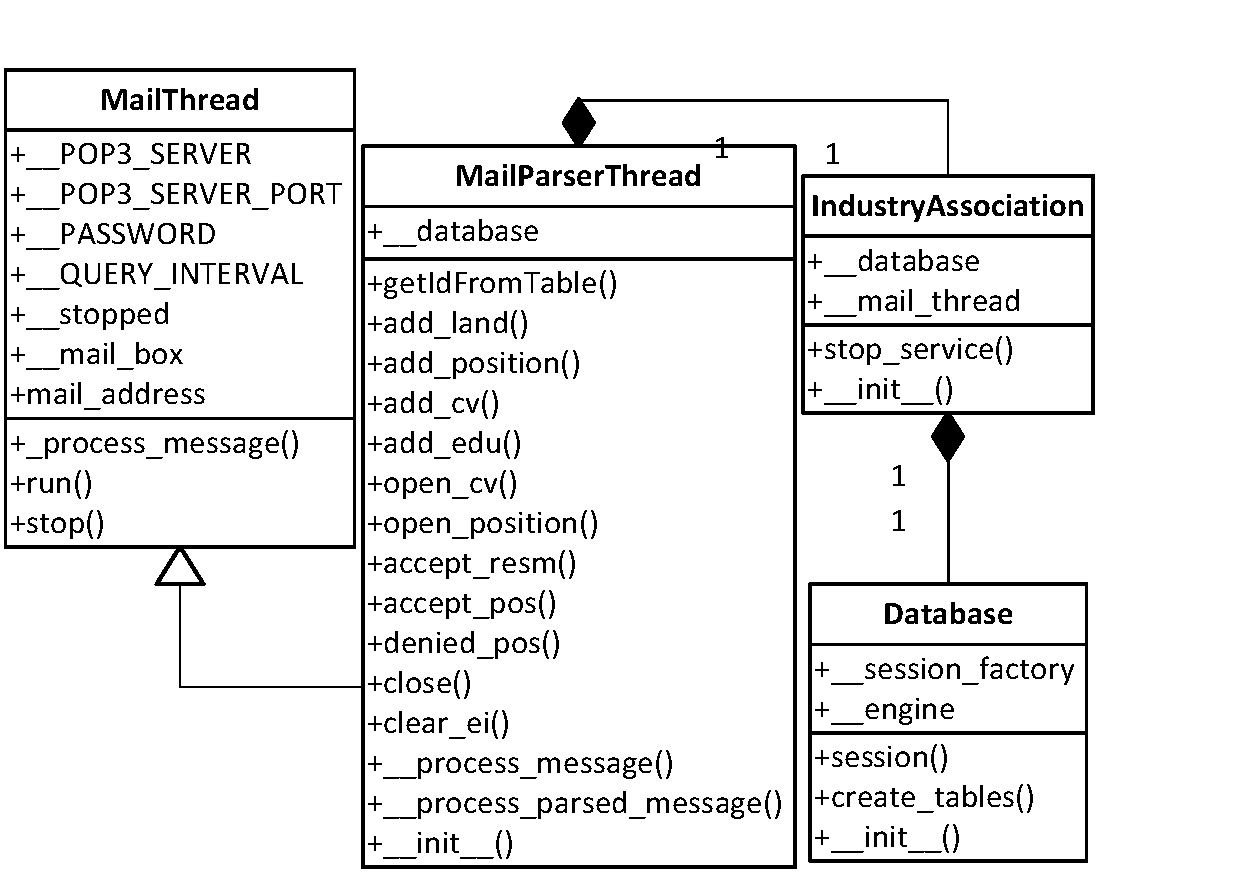
\includegraphics[width=\textwidth]{include/Visio-ia-uml.pdf}
\caption{Диаграмма классов системы отраслевой организации}
\label{fig:Visio-ia-uml}
\end{figure}

Ниже приведена спецификация классов отраслевой организации.

\textbf{Спецификация классов отраслевой организации}
\begin{itemize}
\item Database – класс, реализующий прием электронных писем по протоколу POP3.
	\begin{itemize}
	\item create_tables – метод, создающий таблицы из метаданных объектов;
	\item session – метод, сбрасывает все оставшиеся изменения в базу и фиксирует транзакции, в случае неудачи откатывает сессию;
	\end{itemize}	
\item MailThread – класс, реализующий прием электронных писем по протоколу POP3.
	\begin{itemize}
	\item _process_message – метод, переопределяемый в классах-потомках;                                                                   
	\item run – метод запускающий процесс периодической проверки почтового ящика;
	\item stop – метод останавливающий процесс периодической проверки почтового ящика;
	\end{itemize}
\item MailParserThread – класс, унаследованный от MailThread, обрабатывает входящие электронные письма.
	\begin{itemize}
	\item _process_message - метод принимающий письма и получающий из них отправителя и содержимое;     
	\item \underline{ }\underline{ }process_parsed_message - метод обрабатывающий содержимое писем и, в соответствии с полученными данными, изменяющий информацию о доступных вакансиях;
	\end{itemize}
	
\end{itemize}

\subsubsection{Диаграмма класса, находящегося на узле отраслевой организации, используемого для подбора вакансий}
Диаграмма класса, используемого для подбора вакансий изображена на рисунке ~\ref{fig:Visio-asch-uml}.  
\begin{figure}[ht!]
\centering
 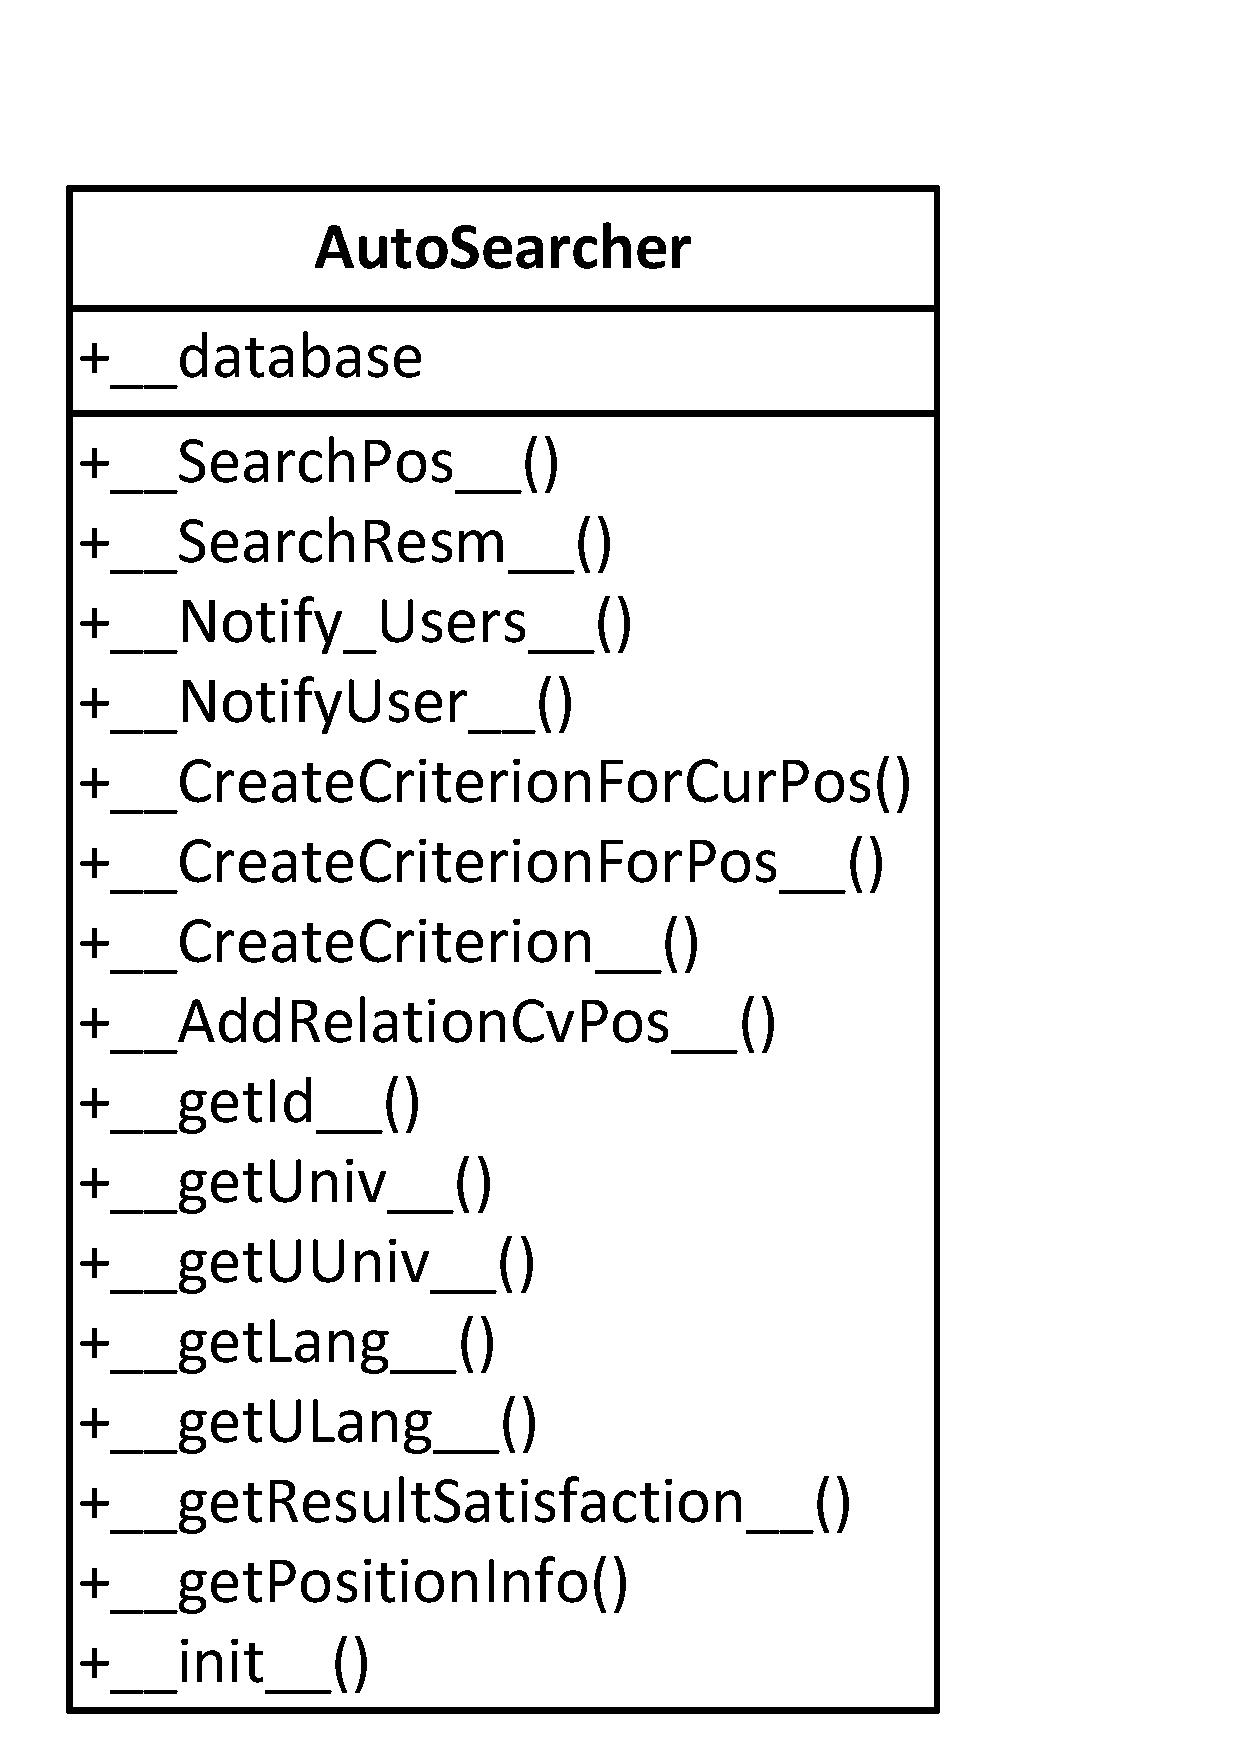
\includegraphics[width=0.5\textwidth]{include/Visio-asch-uml.pdf}
\caption{Диаграмма класса, используемого для подбора вакансий}
\label{fig:Visio-asch-uml}
\end{figure}

Ниже приведена спецификация класса, используемого для подбора вакансий.

\textbf{Спецификация класса, используемого для подбора вакансий}
\begin{itemize}
\item \underline{ }\underline{ }SearchPos\underline{ }\underline{ } – метод, составляющий для кандидатов список вакансий из позиций, для которых критерий схожести с резюме не меньше 0.4;
\item \underline{ }\underline{ }SearchResm\underline{ }\underline{ } – метод, составляющий для вакансии список кандидатов, для которых критерий схожести с резюме не меньше 0.4;
\item \underline{ }\underline{ }Notify_Users\underline{ }\underline{ } – метод, отправляющий письма в по smtp в соответствующие кадровые агентства с идентификаторами подходящих пользователей и описанием вакансии;
\item \underline{ }\underline{ }NotifyUser\underline{ }\underline{ } – метод, отправляющий письмо по smtp в соответствующее кадровое агентство с идентификатором пользователя и описаниями подходящих для него вакансий;
\item \underline{ }\underline{ }CreateCriterionForCurPos – метод, вычисляющий критерий схожести для текущей позиции;
\item \underline{ }\underline{ }CreateCriterionForPos\underline{ }\underline{ } – метод, собирающий все необходимые базы всех резюме и вызывающий метод  \underline{ }\underline{ }CreateCriterionForCurPos для каждого из них и для новой вакансии;
\item \underline{ }\underline{ }CreateCriterion\underline{ }\underline{ } – метод, собирающий все необходимые базы всех вакансий и вызывающий метод  \underline{ }\underline{ }CreateCriterionForCurPos для каждой из них и для нового резюме;
\item \underline{ }\underline{ }AddRelationCvPos\underline{ }\underline{ } – метод, изменяющий статус отклика соискателя на вакансию;
\item \underline{ }\underline{ }getId\underline{ }\underline{ } – метод, получает id строки таблицы по name (только для тех таблиц, в которых данное поле есть);
\item \underline{ }\underline{ }getUniv\underline{ }\underline{ } – метод, получает массив университет и массив специальностей, перечисленных в вакансии;
\item \underline{ }\underline{ }getUUniv\underline{ }\underline{ } – метод, получает массив университет и массив специальностей, перечисленных в резюме;
\item \underline{ }\underline{ }getLang\underline{ }\underline{ } – метод, получает массив иностранных языков и массив уровней подготовки по ним, перечисленных в вакансии 
\item \underline{ }\underline{ }getULang\underline{ }\underline{ } – метод, получает массив иностранных языков и массив уровней подготовки по ним, перечисленных в резюме;
\item \underline{ }\underline{ }getResultSatisfaction\underline{ }\underline{ } – метод, принимающий для сравнения две строки, возвращает true, если отношение совпадающих слов к количеству слов в первой строке больше 0.4;
\item \underline{ }\underline{ }getPositionInfo – метод, формирующий текст - информацию о вакансии для дальнейшей отправки ее в кадровые агентства и просмотра соискателями;

\end{itemize}

\section{Развертывание системы} 
Технические требования к серверам:
Процессор: Pentium III 500 MHz;
ОЗУ: 128 Мбайт;
OC: Linux, Windows, Mac OS;
Программное обеспечение: Python 2.7, SQLAlchemy, CherryPy

На клиентском компьютере должен быть установлен веб-браузер, а разрешение экрана не менее 800x600 точек на дюйм.

\section{Тестирование системы} 
Для проверки работоспособности системы было проведено тестирование функциональных возможностей системы.

\begin{longtable}[ht]{|p{3,5cm}|p{3,5cm}|p{3,5cm}|p{3,5cm}|}
\caption{Результаты тестирования}\label{tab:tab-test-results} \\
\hline
Информация о тесте & Описание теста & Ожидаемый результат  & Результат \\
\hline\hline\endfirsthead
\caption{Результаты тестирования (продолжение)} \\
\hline
Информация о тесте & Описание теста & Ожидаемый результат  & Результат \\
\hline\hline\endhead
\hline
\multicolumn{4}{c}{\textit{Продолжение на следующей странице}}
\endfoot
\endlastfoot
Проверка работы регистрации & Ввод корректных данных & Успешная регистрация в системе & Успешно \\
\hline
Проверка работы регистрации & Ввод зарегистрированного в системе логина& Сообщение, о том, что e-mail уже зарегистрирован & Успешно \\
\hline
Проверка работы регистрации & Незаполненные поля& Сообщение, о том, что некоторые поля пусты & Успешно \\
\hline
Проверка работы авторизации & Ввод верного логина и пароля & Успешный вход в систему & Успешно \\
\hline
Проверка работы авторизации & Ввод незарегистрированного в системе логина или неверного пароля & Сообщение, о ошибке в e-mail или пароле & Успешно \\
\hline
Проверка создания резюме  & Ввод корректных данных & Успешное создание резюме & Успешно \\
\hline
Проверка создания вакансии  & Ввод корректных данных & Успешное создание вакансии & Успешно \\
\hline
Проверка заполнения данных об образовании & Ввод корректных данных & Успешное сохранение данных об образовании & Успешно \\
\hline
Проверка заполнения данных об образовании & Повтор университета и специальности &  Сообщение о дублировании образования & Успешно \\
\hline
Проверка заполнения данных о владении иностранными языками & Ввод корректных данных & Успешное сохранение данных о владении языками & Успешно \\
\hline
Проверка заполнения данных о владении иностранными языками & Повтор наименования языка &  Сообщение о дублировании & Успешно \\
\hline
Проверка создания вакансий  & Ввод корректных данных & Успешное создание вакансий & Успешно \\
\hline
Проверка отправки сообщений отраслевым организациям от компании-нанимателя  & Отправка вакансий для поиска сотрудников & Система отраслевой организации запускает поиск и информирует найденных сотрудников о новой вакансии & Успешно \\
\hline
Проверка отправки сообщений отраслевым организациям от кадрового агентства  & Отправка резюме для поиска вакансий & Система отраслевой организации запускает поиск и информирует сотрудник о подходящих вакансиях & Успешно \\
\hline
Проверка обновления информации & Закрыть вакансию & Система отраслевой организации удаляет вакансию из списка и сигнализирует подписанным пользователям о закрытии указанной заявки & Успешно \\
\hline
\end{longtable}


























